\documentclass[../TinyBot.tex]{subfiles}
\begin{document}

\section{Intro to Programming}

This section will briefly explain what programming is. If you have programmed before, or feel
confident in your programming knowledge, feel free to skip to the \href{sec:introarduino}{next section}.


If you have 0 programming experience and are very confused by this section you may find it
worthwhile to google programming guides and tutorials to really help you understand how to
code and how the code works. There are some links you may find useful at the end of this section. \\


Programming is how we tell computers what we want them to do. We can program a computer to blink a
light, play a noise every time something comes too close, or drive a robot around. The set of
instructions we write is called code, hence why programming is also called coding. Like with spoken
languages, there are many different programming languages. Popular languages include Java, C++,
and Python. This guide will be introducing the Arduino implementation of C++. \\

Each coding language has a set of keywords and special characters that must be used, called ``syntax''.
For the computer to understand your code, it must conform to the expected syntax exactly.
Syntax errors occur when the syntax is not followed, such as there being an unecessary comma,
a letter in the wrong case, an extra bracket, etc. \\

The computer will tell you when there's a syntax error, and will often tell you what line
the error is on. Sometimes this line number is a bit off due to the complexity of the syntax;
the syntax error might be a few lines above the specified line. When you first start coding,
noticing where there is a syntax error is quite difficult; however, as with many things,
as you get more used to programming you get better at noticing and guessing where a syntax error is. \\ 

A crucial part of programming is saving data so it can be used later. Variables are the simplest way
of saving data. Since C++ is a strong typed language, you need to tell the computer exactly what type
of data the computer is being told to remember.\\

Here we tell the computer to remember an \lstinline[]!int!eger variable called \lstinline[]!number1!
which has the value 4.
\begin{lstlisting}
int number1 = 4;
\end{lstlisting}

The keyword \lstinline[]!int! is really important, it tells the computer that the variable
\lstinline[]!number1! is an integer (a whole number, negative, positive, or 0). \\

Some other basic datatypes include:
\begin{itemize}[label={$\triangleright$}]
  \item \lstinline[]!float! - a decimal number such as 0.5, 3.14159, etc. 
  \item \lstinline[]!char! - a character, such as 'a' or '2' - note the single quotation marks which are important when declaring (creating) a character variable
  \item \lstinline[]!string! - a sequence of characters e.g. "hello world" or "this is a string"; double quotation marks are essential for strings in C++. 
\end{itemize}

These datatypes are a common concept across many languages, though some languages, like Python,
don't require you to explicitly state what datatype a variable is (known as a weak typed language). \\

Some more C++ resources:
\begin{itemize}[label={$\triangleright$}]
  \item \href{https://www.w3schools.com/cpp/default.asp}{https://www.w3schools.com/cpp/default.asp}
  \item \href{https://www.learncpp.com/}{https://www.learncpp.com/}
\end{itemize}

\section{Intro To Arduinos} \label{sec:introarduino}

To program an Arduino, you will need a USB cable, and a laptop/desktop with the
\href{https://www.arduino.cc/en/software}{Arduino IDE} installed, IDE stands for
``Integrated Development Environment''. \\

\begin{figure}[h]
    \centering
    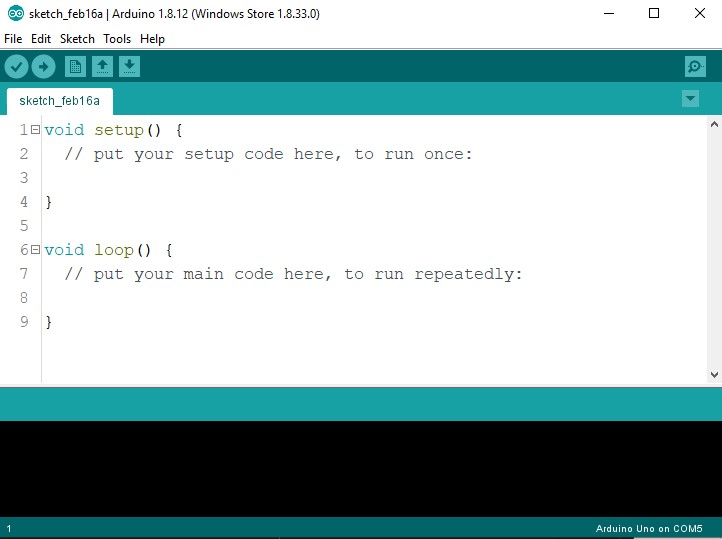
\includegraphics[width=0.7\textwidth]{arduino_ide.jpg}
    \caption{The Arduino IDE}
\end{figure}

The two round buttons in the top right, the tick and the arrow, are the verify and upload buttons.
Verify checks your code, making sure that the syntax (think of it like a grammar checker) of
your code is correct. Upload sends the code you've written to the Arduino board, if it can be verified.  \\

However, before you can upload your code you need to select the Arduino board being used, as shown below.

\begin{center}
  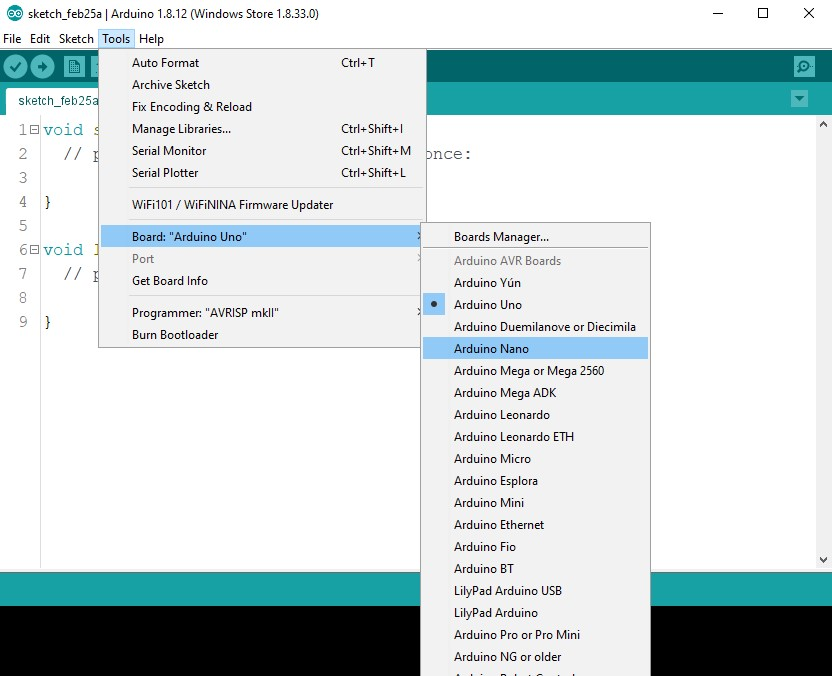
\includegraphics[width=0.6\textwidth]{arduino_ide_select_board.jpg}
  \captionof{figure}{Selecting the Board}
\end{center}

Next, you need to select the USB port that the Arduino is connected to. This is also done
through the Tools menu. The port should appear as COM followed by a number. This number
will change depending on which USB port the Arduino is plugged into. If the port option is
greyed out for you, try plugging the Arduino into a different USB port. 

\begin{center}
  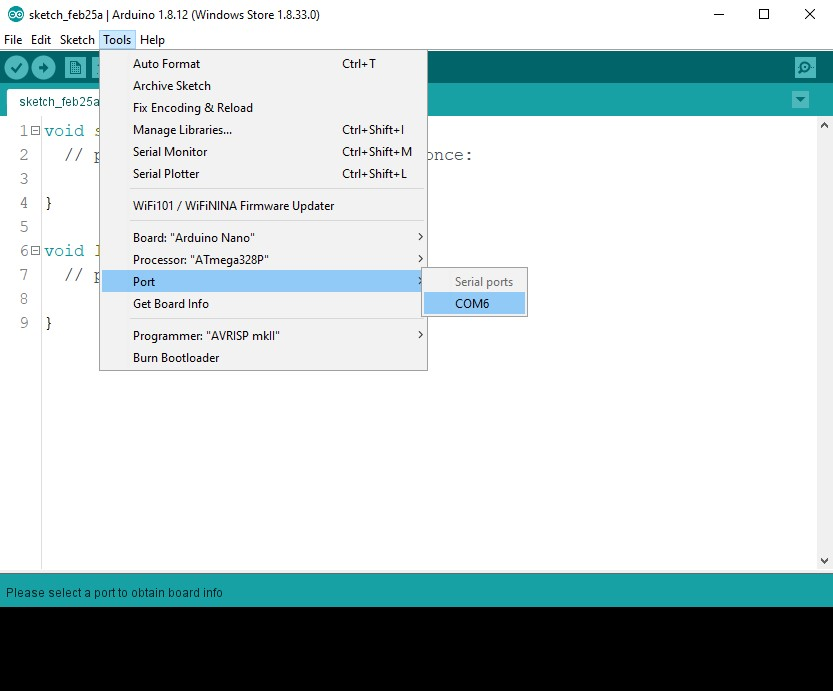
\includegraphics[width=0.6\textwidth]{arduino_ide_select_port.jpg}
  \captionof{figure}{Selecting Port}
\end{center}

\bigskip

Arduino's are programmed in the programming language \lstinline[]!C++!, though there
are a few differences. The below code section details a few features of coding.

\begin{lstlisting}
// this is a comment, comments are not read by the computer and can be anything you want

// variables declared not in a function will be accessible
// in all functions
int global_var = 0;

void setup {
  // everything in this function will run once

  // this code will run when the board is powered on,
  // or when the reset button is pressed
}

void loop {
  // everything in this function will run repeatedly
}

\end{lstlisting}
\bigskip

\pagebreak
A useful feature of the Arduino IDE is all the example code which is provided.

\begin{center}
    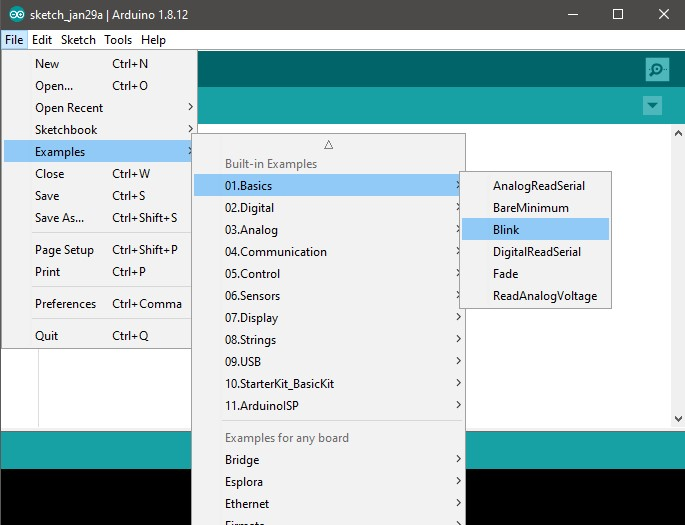
\includegraphics[width=0.7\textwidth]{arduino_ide_blink_example.jpg}
    \label{fig:ide-blink}
    \captionof{figure}{Arduino IDE Example Code}
\end{center}

The simplest Arduino example is the Blink code, which turns on and off an onboard LED.

\begin{lstlisting}
void setup() {
  // initialize digital pin LED_BUILTIN as an output.
  pinMode(LED_BUILTIN, OUTPUT);
}

// the loop function runs over and over again forever
void loop() {
  // turn the LED on (HIGH is the voltage level)
  digitalWrite(LED_BUILTIN, HIGH); 

  delay(1000);      // wait for a second

  // turn the LED off by making the voltage LOW
  digitalWrite(LED_BUILTIN, LOW);  
  
  delay(1000);      // wait for a second
}
\end{lstlisting}


There are a few common aspects present in the code of nearly every Arduino project, no
matter how simple or complicated. \\

\lstinline[]!pinMode(<pin number>, <mode>)! sets a digital pin on the Arduino to be either
an \lstinline[]!INPUT! or and \lstinline[]!OUTPUT!. \\

\lstinline[]!digitalWrite()! is used to set digital pins \lstinline[]!HIGH! and \lstinline[]!LOW!.

\end{document}